% Mahfuzur Rahman Khan - Backend Lead Engineer CV
\documentclass[10pt,a4paper]{article}

\usepackage[utf8]{inputenc}
\usepackage[T1]{fontenc}
\usepackage[margin=1.15cm]{geometry}
\usepackage[hidelinks]{hyperref}
\usepackage{array}
\usepackage{tabularx}
\usepackage{graphicx}
\IfFileExists{fontawesome5.sty}{%
  \usepackage{fontawesome5}
  \newcommand{\contacticon}[1]{\makebox[1.15em][c]{\faIcon{#1}}}
}{%
  \newcommand{\contacticon}[1]{}
}

\pagestyle{empty}
\setlength{\parindent}{0pt}
\setlength{\parskip}{0pt}
\setlength{\tabcolsep}{0pt}
\renewcommand{\arraystretch}{0.98}

\newcommand{\cvsection}[1]{%
  \vspace{0.55em}
  {\normalsize\bfseries\MakeUppercase{#1}}\par
  \vspace{0.12em}\hrule\vspace{0.28em}
}

\newcommand{\roleentry}[4]{%
  \textbf{#1} \hfill \textbf{#2}\\
  \textit{#3} \hfill \textit{#4}\par\vspace{-0.12em}
}

\newcommand{\projectentry}[3]{%
  \textbf{#1} -- #2\\
  \textit{#3}\par\vspace{0.12em}
}

\newenvironment{cvitems}{%
  \begin{itemize}
    \setlength{\itemsep}{0.03em}
    \setlength{\parskip}{0pt}
    \setlength{\parsep}{0pt}
    \setlength{\topsep}{0.08em}
    \setlength{\leftmargin}{1.2em}
}{\end{itemize}}

\begin{document}
\fontsize{9.5}{10.8}\selectfont

\noindent
\begin{minipage}[t]{0.76\textwidth}
\vspace{0pt}
{\LARGE \textbf{Mahfuzur Rahman Khan}}\\[0.18em]
{\large Backend Lead Engineer}\\[0.18em]
\contacticon{map-marker-alt}Dhaka, Bangladesh\\
\contacticon{envelope}\href{mailto:mahfuzku11@gmail.com}{mahfuzku11@gmail.com}\\
\contacticon{mobile-alt}+8801520103197\\
\contacticon{linkedin}\href{https://www.linkedin.com/in/mahfuz110244}{linkedin.com/in/mahfuz110244} \textbar{}
\contacticon{github}\href{https://github.com/mahfuz110244}{github.com/mahfuz110244} \textbar{}
\contacticon{globe}\href{https://mr-khan.gitlab.io/}{mr-khan.gitlab.io}
\end{minipage}
\hfill
% ===== PHOTO -- included by choice. Common/expected for BD, EU, Asia & MENA CVs.
% ===== Heads-up: many US/UK/CA/AU employers and some ATS prefer no photo. =====
\begin{minipage}[t]{0.18\textwidth}
\vspace{-0.28cm}
\raggedleft
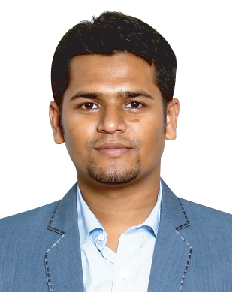
\includegraphics[width=2.6cm,height=3.0cm,keepaspectratio]{mrk}
\end{minipage}

\cvsection{Professional Summary}
Backend Lead Engineer with \textbf{10+ years of experience} designing, modernizing, and scaling distributed systems, microservices, and payment platforms across \textbf{EdTech, FinTech, E-commerce, Logistics, and SaaS}. Currently lead backend engineering at \textbf{Shikho}, Bangladesh's largest EdTech platform (\textbf{3M+ learners}). Deep in Golang and system design, with a track record in legacy modernization, production reliability, team mentoring, and AI-assisted engineering workflows.

\cvsection{Core Skills}
\begin{tabularx}{\textwidth}{>{\bfseries}p{3.3cm}@{\hspace{0.6em}}X}
Leadership & Backend team leadership, mentoring, architecture reviews, code reviews, technical planning, cross-functional delivery, incident analysis\\
Architecture & Microservices, distributed systems, event-driven architecture, clean architecture, CQRS, API design, legacy modernization\\
Backend & Golang, Python, TypeScript, JavaScript, REST APIs, GraphQL, gRPC, Django REST Framework, FastAPI, NestJS, Echo\\
Data \& Messaging & PostgreSQL, MongoDB, MySQL, DynamoDB, Redis, Elasticsearch, ArangoDB, RabbitMQ, Kafka, NATS\\
Cloud \& DevOps & AWS, Docker, Kubernetes, Nginx, Linux, CI/CD, observability, performance optimization\\
AI Productivity & Spec-driven development, context engineering, AI-augmented code review, automated test \& documentation generation; tooling: Claude Code, OpenAI Codex, Gemini CLI
\end{tabularx}

\cvsection{Career Highlights}
\begin{cvitems}
  \item Lead backend engineering at \textbf{Shikho} (\textbf{3M+ learners}), setting architecture and delivery standards across an \textbf{8-member backend team} within a \textbf{30+ engineer} organization.
  \item Architected and shipped \textbf{20+ production microservices} spanning payments, wallet, enrollment, and content platforms [ADD METRIC: e.g., sustaining \textasciitilde N req/s at 99.9\% uptime].
  \item Led monolith-to-microservices migrations and payment-orchestration platforms [ADD METRIC: e.g., cutting deployment time \textasciitilde X\% / reducing infra cost \textasciitilde Y\%].
\end{cvitems}

\cvsection{Professional Experience}
\roleentry{Backend Lead Engineer}{Jan 2025 -- Present}{Shikho}{Banani, Dhaka}
\begin{cvitems}
  \item Own backend architecture and delivery across learning, enrollment, payments, content delivery, and operations for Bangladesh's largest EdTech platform.
  \item Provide technical leadership across \textbf{30+ engineers} while directly leading an \textbf{8-member backend team}.
  \item Design and maintain production Golang microservices focused on scalability, reliability, and maintainability [ADD METRIC: e.g., serving \textasciitilde N req/s across core services].
  \item Drive backend modernization through API refactoring, service decomposition, and platform optimization, improving [ADD METRIC: e.g., p99 latency / reliability], with rigorous architecture review, code review, and incident analysis.
  \item Apply \textbf{Claude Code, OpenAI Codex, and Gemini CLI} to accelerate delivery, test generation, and documentation while keeping design and review human-led.
\end{cvitems}

\roleentry{Senior Software Engineer}{Jul 2024 -- Dec 2024}{Supertal Pte. Ltd.}{Singapore}
\begin{cvitems}
  \item Served as lead backend engineer for the \textbf{Hypermart Backend Team}, supporting a large Indonesian grocery retail chain.
  \item Built core, discount, and seller APIs using \textbf{Golang, MongoDB, MySQL, Elasticsearch, and Redis}; refactored legacy services to improve maintainability and stability [ADD METRIC: e.g., cut p95 latency / defect rate by X\%].
\end{cvitems}

\roleentry{SDE-II Golang Engineer, Team Lead -- Bohubrihi}{Apr 2022 -- Jun 2024}{Shikho}{Banani, Dhaka}
\begin{cvitems}
  \item Led the \textbf{Bohubrihi Backend Team}, owning \textbf{7 production microservices} across learners, instructors, enrollment, content, and operations.
  \item Drove migration of the Bohubrihi WordPress monolith to a scalable microservices architecture [ADD METRIC: e.g., enabling independent deploys / improving uptime or page-load by X].
  \item Mentored engineers on clean architecture, code quality, and review practices, raising delivery consistency across the team.
\end{cvitems}

\roleentry{Senior Software Engineer}{Nov 2021 -- Mar 2022}{Gononet Ltd.}{Gulshan, Dhaka}
\begin{cvitems}
  \item Designed and developed \textbf{GorillaMove} grocery delivery microservices covering core, inventory, and sales workflows.
  \item Delivered \textbf{Choukash ERP} microservices for Gononet LLC, USA, and guided junior engineers across parallel projects.
\end{cvitems}

\roleentry{Software Engineer}{Feb 2021 -- Sep 2021}{Evaly Ltd.}{Dhanmondi, Dhaka}
\begin{cvitems}
  \item Built a high-throughput wallet microservice for balance payments, refunds, and cashbacks serving millions of users [ADD METRIC: e.g., \textasciitilde N TPS / \$X monthly volume].
  \item Built payment-orchestration integrations with \textbf{bKash, Nagad, SSLCommerz, Balance, and Gift Card}; optimized queries and caching to reduce AWS cost [ADD METRIC: e.g., by \textasciitilde X\%] and improve response times.
\end{cvitems}

\roleentry{Senior Software Engineer}{Sep 2020 -- Jan 2021}{Dingi Technologies Ltd.}{Gulshan, Dhaka}
\begin{cvitems}
  \item Designed a multi-tenant SaaS platform using Django REST Framework, Elasticsearch geofence search, caching, and AWS-backed services.
\end{cvitems}

\roleentry{Software Engineer}{May 2019 -- May 2020}{Misfit Technologies Ltd.}{Banani, Dhaka}
\begin{cvitems}
  \item Led backend delivery for a real-time chatbot platform with Facebook/WhatsApp APIs, appointment booking, rescheduling, and queue-management workflows.
\end{cvitems}

\roleentry{Software Engineer / Junior Software Engineer}{Jul 2016 -- Apr 2019}{Brain Station 23 Ltd.}{Mohakhali, Dhaka}
\begin{cvitems}
  \item Developed backend/full-stack features for health management, entrepreneurship, ERP, and enterprise applications; built Odoo modules and supported sprint delivery.
\end{cvitems}

\cvsection{Selected Projects}
\projectentry{Shikho}{Large-scale EdTech platform serving \textbf{3M+ learners}; led backend architecture and delivery for learning, enrollment, payments, content delivery, and operations.}{Golang, MongoDB, PostgreSQL, Redis, RabbitMQ, Docker, gRPC, GraphQL}
\projectentry{Bohubrihi}{Online learning platform migrated from WordPress monolith to \textbf{7 production microservices}; led backend service decomposition and delivery.}{Golang, MongoDB, PostgreSQL, Redis, RabbitMQ, NATS, Docker, GraphQL}
\projectentry{Hypermart}{Backend services for a large Indonesian grocery retail chain; developed core, discount, and seller APIs and improved legacy API quality.}{Golang, MongoDB, MySQL, Elasticsearch, Redis}
\projectentry{Evaly Wallet \& Payments}{High-throughput wallet and payment orchestration platform integrating bKash, Nagad, SSLCommerz, Balance, and Gift Cards.}{Golang, Python, Django REST Framework, PostgreSQL, Redis, RabbitMQ, Docker}
\projectentry{GorillaMove \& Choukash ERP}{Grocery delivery and ERP microservices covering core, inventory, sales, order processing, and operational workflows.}{Golang, Echo, PostgreSQL, Docker, Algolia}
\projectentry{FollowR \& Lily}{Fleet-management SaaS with geofence search, and a real-time Facebook/WhatsApp chatbot platform featuring appointment booking and OCR-based NID verification.}{Python, Django REST Framework, FastAPI, PostgreSQL, AWS, Elasticsearch, Celery, Redis, Vue.js}

\cvsection{Education}
\roleentry{BSc. in Computer Science and Engineering}{2011 -- 2015}{Khulna University}{Khulna, Bangladesh}
CGPA: 3.55 / 4.00

\cvsection{Certifications}
\begin{cvitems}
  \item Golang Certification -- Mangtas, 2022
  \item AWS Business Professional; AWS TCO and Cloud Economics, 2018
  \item AWS Technical Professional, 2017
\end{cvitems}

\cvsection{Publication}
\textbf{Mahfuzur Rahman Khan}, ABM Muhitur Rahman, G M Atiqur Rahaman and Md Abul Hasnat, ``Unsupervised RGB-D Image Segmentation by Multi-layer Clustering,'' \textit{IEEE International Conference on Informatics, Electronics \& Vision (ICIEV)}, 2016.
\href{https://ieeexplore.ieee.org/document/7760095/}{Link}

\cvsection{Profiles}
\href{https://mr-khan.gitlab.io/}{Personal Blog} \textbar{}
\href{https://medium.com/@mahfuz110244}{Medium} \textbar{}
\href{https://github.com/mahfuz110244}{GitHub} \textbar{}
\href{http://stackoverflow.com/users/2713054/mahfuz110244}{Stack Overflow} \textbar{}
\href{https://www.hackerrank.com/mahfuz110244}{HackerRank} \textbar{}
UVA Online Judge ID: 140086

\end{document}
